% OLS on the same 20 observations: intercept=-0.127313769752, slope=0.124153498871.
% Native PGFPlots; reproduced by examples/generate_foundation_figures.py.
% Constructed observations / analytical teaching example, not empirical data.
\begingroup
\definecolor{blueplot}{HTML}{4E79A7}
\definecolor{redplot}{HTML}{D95F59}
\definecolor{inkplot}{HTML}{111111}
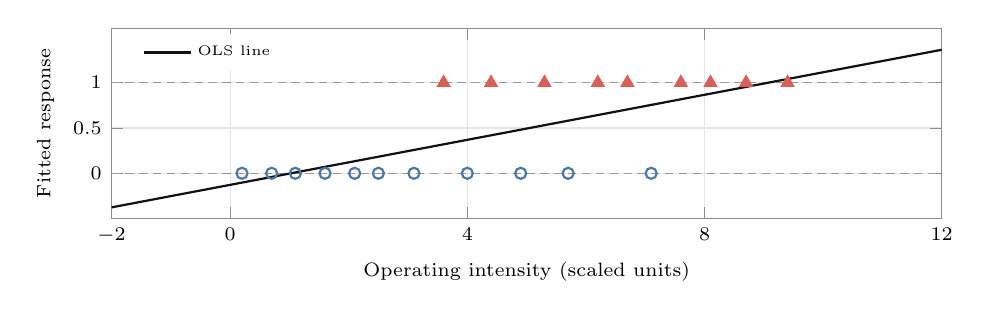
\begin{tikzpicture}
\begin{axis}[
width=\linewidth,height=4.0cm,font=\scriptsize,
tick label style={font=\scriptsize},label style={font=\scriptsize},
axis line style={black!45},tick style={black!45},
grid=major,grid style={black!10},scaled ticks=false,
clip=true,unbounded coords=jump,
legend style={font=\tiny,draw=none,fill=white,fill opacity=.94,text opacity=1,
  legend cell align=left,inner sep=2pt,row sep=1pt},
xmin=-2,xmax=12,ymin=-.5,ymax=1.6,
xlabel={Operating intensity (scaled units)},ylabel={Fitted response},
xtick={-2,0,4,8,12},ytick={0,.5,1},legend pos=north west
]
\addplot[black!40,densely dashed,no marks,forget plot] coordinates {(-2,0) (12,0)};
\addplot[black!40,densely dashed,no marks,forget plot] coordinates {(-2,1) (12,1)};
\addplot[inkplot,thick,no marks] coordinates {(-2,-0.3756207675) (12,1.362528217)};
\addlegendentry{OLS line}
\addplot[blueplot,only marks,mark=o,mark size=2.0pt,thick,forget plot] coordinates {(0.2,0) (0.7,0) (1.1,0) (1.6,0) (2.1,0) (2.5,0) (3.1,0) (4,0) (4.9,0) (5.7,0) (7.1,0)};
\addplot[redplot,only marks,mark=triangle*,mark size=2.6pt,forget plot] coordinates {(3.6,1) (4.4,1) (5.3,1) (6.2,1) (6.7,1) (7.6,1) (8.1,1) (8.7,1) (9.4,1)};

\end{axis}
\end{tikzpicture}
\endgroup
